\section{Image representation}

In BoW model each image is represented as a histogram of \emph{visual words} occurrences through local descriptor quantization\cite{DBLP:journals/corr/abs-1304-5168}. These histograms are used to train an image category classifier.

To quantize local descriptors into visual words, we must first generate visual vocabulary. 

\subsection{Vocabulary creation}

The visual vocabulary for BoW model is often generated by clustering of images local descriptors. In this case we \emph{k-means} algorithm as clustering method.

This algorithm iteratively groups the descriptors into $k$ mutually exclusive clusters, where $k$ is the preset \emph{vocabulary size}. The resulting cluster are compact and separated by similar characteristics so they are trated as a unique visual word from the vocabulary, in which each \emph{codeword} is represented by the centroid of the cluster.

\subsection{Feature quantization}

Feature quantization is the process of assigning one local descriptor to one or multiple
visual words. To assign a descriptor to visual word(s) there are two way to proceed: \emph{hard assignment} or \emph{soft assignment}.

\subsubsection{Hard assignment}

A simple way to assign a descriptor to a visual word is to search for nearest neighbors among the vocabulary.

Let $V = \{\omega_1, \ldots, \omega_n \}$ be the vocabulary, where $\omega_i \in \mathbb{R}^{d}$ (with $d$ the SIFT descriptor vector size, 128) and $n$ is the vocabulary size.

In \emph{hard assignment}, given and image with $X = \{x_1, \ldots, x_p\}$ extracted local features, each local feature $x_i \in \mathbb{R}^{d}$ is assigned to one and only one codeword of the vocabulary. The assigned codeword index, $u_i$, is obtained with

$$u_i = arg \min_{j = 1, \ldots, n} ||x_i - \omega_j||$$

As result we obtain an index vector that associate each local feature with its closest codeword index of the vocabulary.

\subsubsection{Soft assignment}

The \emph{hard assignment} method does not consider codeword ambiguity and often introduces large quantization error. Those two issue are known as \emph{codeword uncertainty} and \emph{codeword plausibility}. 

Codeword uncertainty refers to the problem of selecting the correct codeword out of two or more relevant candidates. The \emph{hard assignment} approach merely selects the best representing codeword, ignoring the relevance of other candidates. 

Codeword plausibility denotes the problem of selecting a codeword without a suitable candidate in the vocabulary. The \emph{hard assignment} approach assigns the best fitting codeword, regardless the fact that this codeword is not a proper representative. 

\begin{figure}[h]
\begin{center}
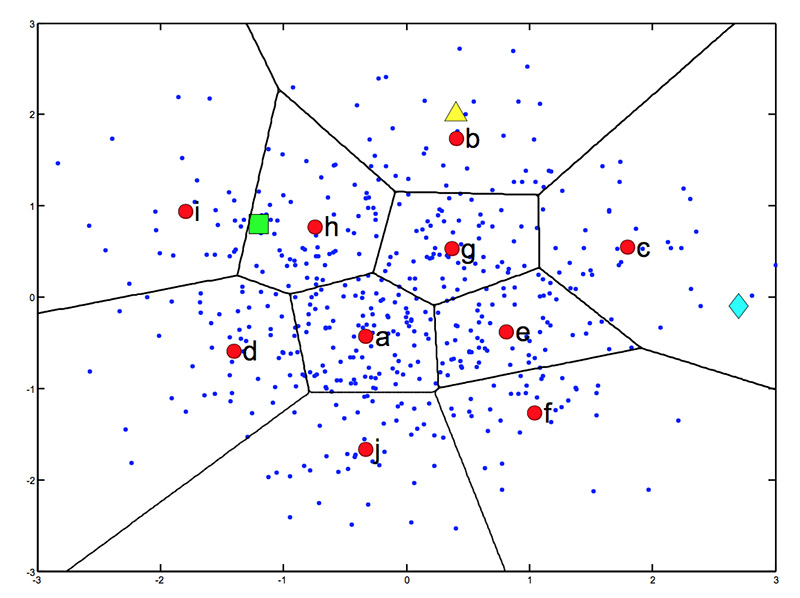
\includegraphics[width=0.35\textwidth]{images/soft-assignment.jpg}
\end{center}
  \caption{\emph{Codeword uncertainty} and \emph{codeword plausibility}}
\label{fig:softAssignment}
\end{figure}

Figure \ref{fig:softAssignment} illustrates both these problems. The small dots represent image features, the labeled red circles are the visual words. The yellow triangle represents a data sample that is well suited to the hard assignment approach. The difficulty with codeword uncertainty is shown by the square, and the problem of codeword plausibility is illustrated by the diamond.

\emph{Soft assignment} coding is proposed to alleviate those drawbacks by assigning a local feature to all visual words. The coding coefficient represents the membership of a local feature to different visual words.

\paragraph{Kernel Codebook}

In Kernel Codebook approach we apply techniques from kernel density estimation to allow a degree of ambiguity in assigning codewords to image features. 

For each local feature $v$ we evaluate
$$KCB(v) = \frac{1}{n} \sum_{i = 1}^{n} K_{\sigma}(D(v, r_i))$$
where $n$ is the number of regions, $r_i$ is the image region $i$ and $K_{\sigma}$ is the kernel function defined as
$$K_{\sigma} (x) = \frac{1}{\sqrt{2\pi} \sigma} e^{- \frac{1}{2} \frac{x^2}{\sigma^2}}$$

In essence Kernel Codebook smoothes the hard mapping of features in an image region to the codeword vocabulary.

\paragraph{Codeword uncertainty}

Codeword uncertainty indicates that one image region may distribute probability mass to more than one codeword.

$$UNC(v) = \frac{1}{n} \sum_{i = 1}^{n} \frac{K_{\sigma}(D(v, r_i))}{\sum_{j=1}^{|V|} K_{\sigma}(D(\omega_j, r_i))}$$

\paragraph{Localized soft assignment}

In the \emph{localized soft assignment} approach, as proposed in an \emph{early cut-off} effect is produced, which removes the adverse impact of unreliable longer distances
